\documentclass{beamer}

\usepackage{amsmath}
\usepackage{amssymb}
\usepackage{amsthm}
\usepackage{mathtools}
\usepackage[UKenglish]{babel}
\usepackage{enumerate}
\usepackage{graphicx}
\usepackage{braket}
\usepackage{esint}
\usepackage{float}
\usepackage{tabularx}
\usepackage{array}
\usepackage{subcaption}
\usepackage{hyperref}
\hypersetup{colorlinks=false, bookmarks=true}

\usetheme{Madrid}
\usecolortheme{seahorse}
\usefonttheme{professionalfonts}
\useinnertheme{circles}

\AtBeginSection[]
{
  \begin{frame}
    \frametitle{Table of Contents}
    \tableofcontents[currentsection]
  \end{frame}
}

\setbeamertemplate{caption}[numbered]

\title[QCNN State Preparation]{A QCNN for Quantum State Preparation}
\subtitle{Carnegie Vacation Scholarship}
\author[David Amorim]{David Amorim}
\institute[]{}
\date[05/08/2024]{Week 5 \\(29/07/2024 - 02/08/2024)}

\begin{document}

\frame{\titlepage}

\section{Preliminaries}
\begin{frame}
\frametitle{Aims for the Week}
The following aims were set at the last meeting (29/07/2024):

\begin{alertblock}{Improve Loss Function}
Work on an improved version of WILL. Incorporate some phase extraction metrics (e.g. $\chi$, $\epsilon$) into the loss function. 
\end{alertblock}

\begin{alertblock}{Investigate Phase Extraction}
Study the relationship between mismatch and the extracted phase, i.e. study the operator $\tilde{Q}^\dagger (\hat{I} \otimes\hat{R}) \tilde{Q}$. 
\end{alertblock}

\begin{alertblock}{Mitigate Barren Plateaus}
Work on strategies to mitigate barren plateaus, e.g. implement layer-by-layer training.
\end{alertblock}
\end{frame}

\section{Improving the Loss Function}

\begin{frame}
\frametitle{WILL Revisited}
\begin{itemize}
\item As discussed at the meeting on 29/07, the definition of \alert{WILL} (weighted L$_\text{p}$ loss) was amended to: 
\begin{equation}
\text{WILL}_\text{p,q} =  \left( \sum_k \Big|x_k -y_k \Big|^p \alert{+ |x_k|} \Big|[k]_m - \Psi([k]_n) \Big|^q \right)^{1/p},
\end{equation}
where the changes to the previous definition are highlighted
\item Testing this for different $\Psi$ (with $L=6$, $m=3$ and 600 epochs) yielded the following optimal values for $p$, $q$:
\end{itemize}
\begin{table}
\centering 
\begin{tabular}{c|c| c}
$\Psi(f)$ & $p$ & $q$ \\ \hline 
$\sim f$ & 0.25 & 0.5  \\
$\sim  f^2$ & 1 & 1.5  \\
$\Psi_{\text{H23}}$ & 0.75 & 2  \\
\end{tabular}
\caption{Optimal identified $p$, $q$ values for WILL}
\end{table}
\end{frame}

\begin{frame}
\frametitle{Comparing SAM, WIM, and WILL}
\begin{columns}
\begin{column}{0.5\textwidth}
\begin{table}
\begin{tabular}{c || c| c| c }
& SAM & WIM & WILL \\ \hline \hline 
$\mu$ &  \textbf{3.4e-2} & 6.0e-2 & 4.5e-1 \\
$\sigma$ &  1.4e-1 &1.1e-1 & 4.7e-1 \\
$\epsilon$  &  \textbf{1.9e-2} & 9.2e-2 & 2.6e-1  \\
$\chi$ & \textbf{ 3.2e-2} & 5.1e-2  & 3.7e-1  \\ \hline 
$\Omega$ &  \textbf{4.46} & 3.19 & 0.76
\end{tabular}
\caption{Comparing loss function metrics for $\Psi(f) \sim f$ ($L=6$, $m=3$, 600 epochs)}
\end{table}
\end{column}
\begin{column}{0.5\textwidth}
\begin{figure}
\centering 
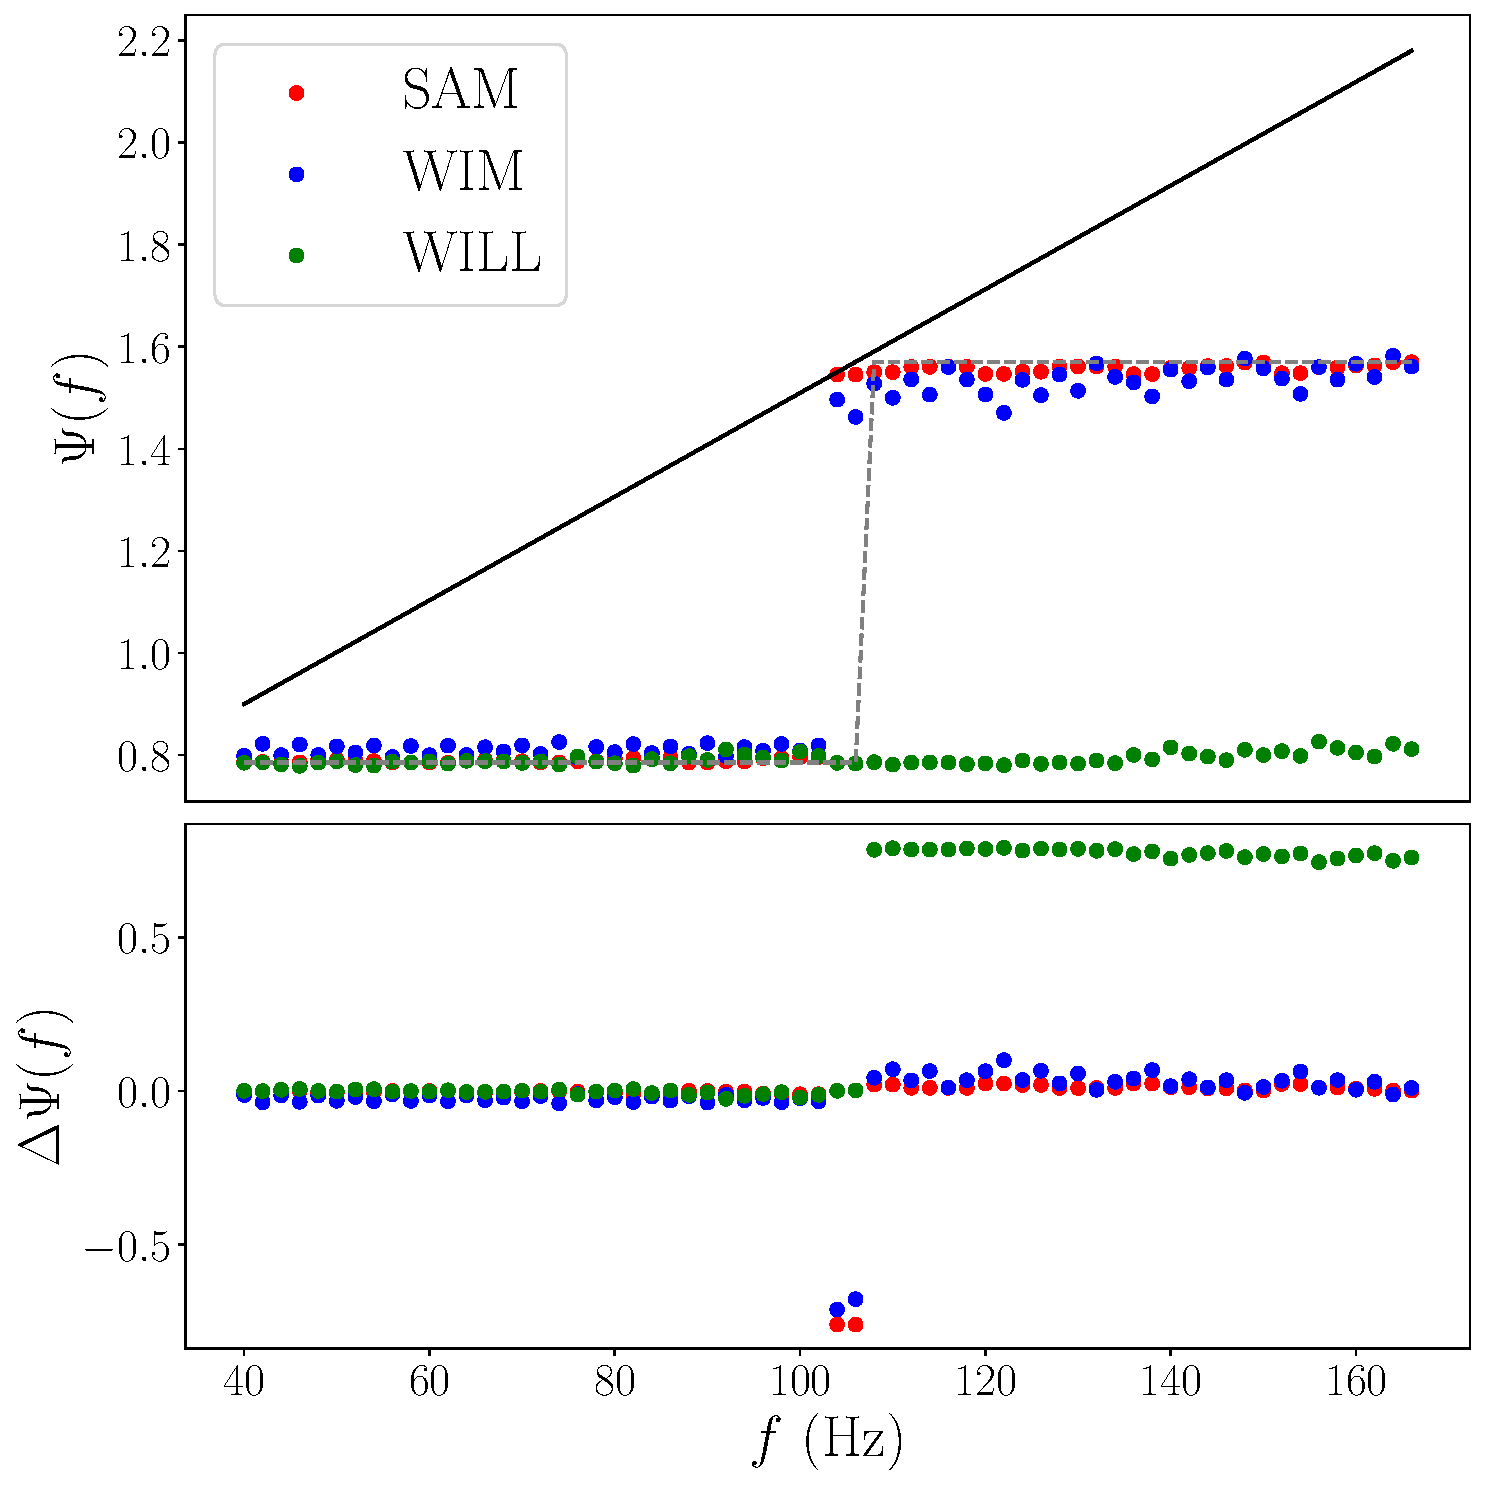
\includegraphics[width=\textwidth]{im/SAM_WIM_WILL_F_new}
\caption{Comparing extracted phase functions for $\Psi(f) \sim f$ ($L=6$, $m=3$, 600 epochs)}
\end{figure}
\end{column}
\end{columns}
\end{frame}

\begin{frame}
\frametitle{Comparing SAM, WIM, and WILL}
\begin{columns}
\begin{column}{0.5\textwidth}
\begin{table}
\begin{tabular}{c || c| c| c }
& SAM & WIM & WILL \\ \hline \hline 
$\mu$ &  \textbf{1.9e-1} & 2.3e-1 & 6.6e-1  \\
$\sigma$ &  1.2e-1 & \textbf{1.0e-1} & 4.1e-1\\
$\epsilon$  &  2.2e-1 & 4.2e-1 & \textbf{2.8e-2}  \\
$\chi$ &  \textbf{1.9e-1} & 2.0e-1 & 6.1e-1  \\ \hline 
$\Omega$ &  \textbf{1.39} & 1.05 & 0.57
\end{tabular}
\caption{Comparing loss function metrics for $\Psi(f) \sim f^2$ ($L=6$, $m=3$, 600 epochs)}
\end{table}
\end{column}
\begin{column}{0.5\textwidth}
\begin{figure}
\centering 
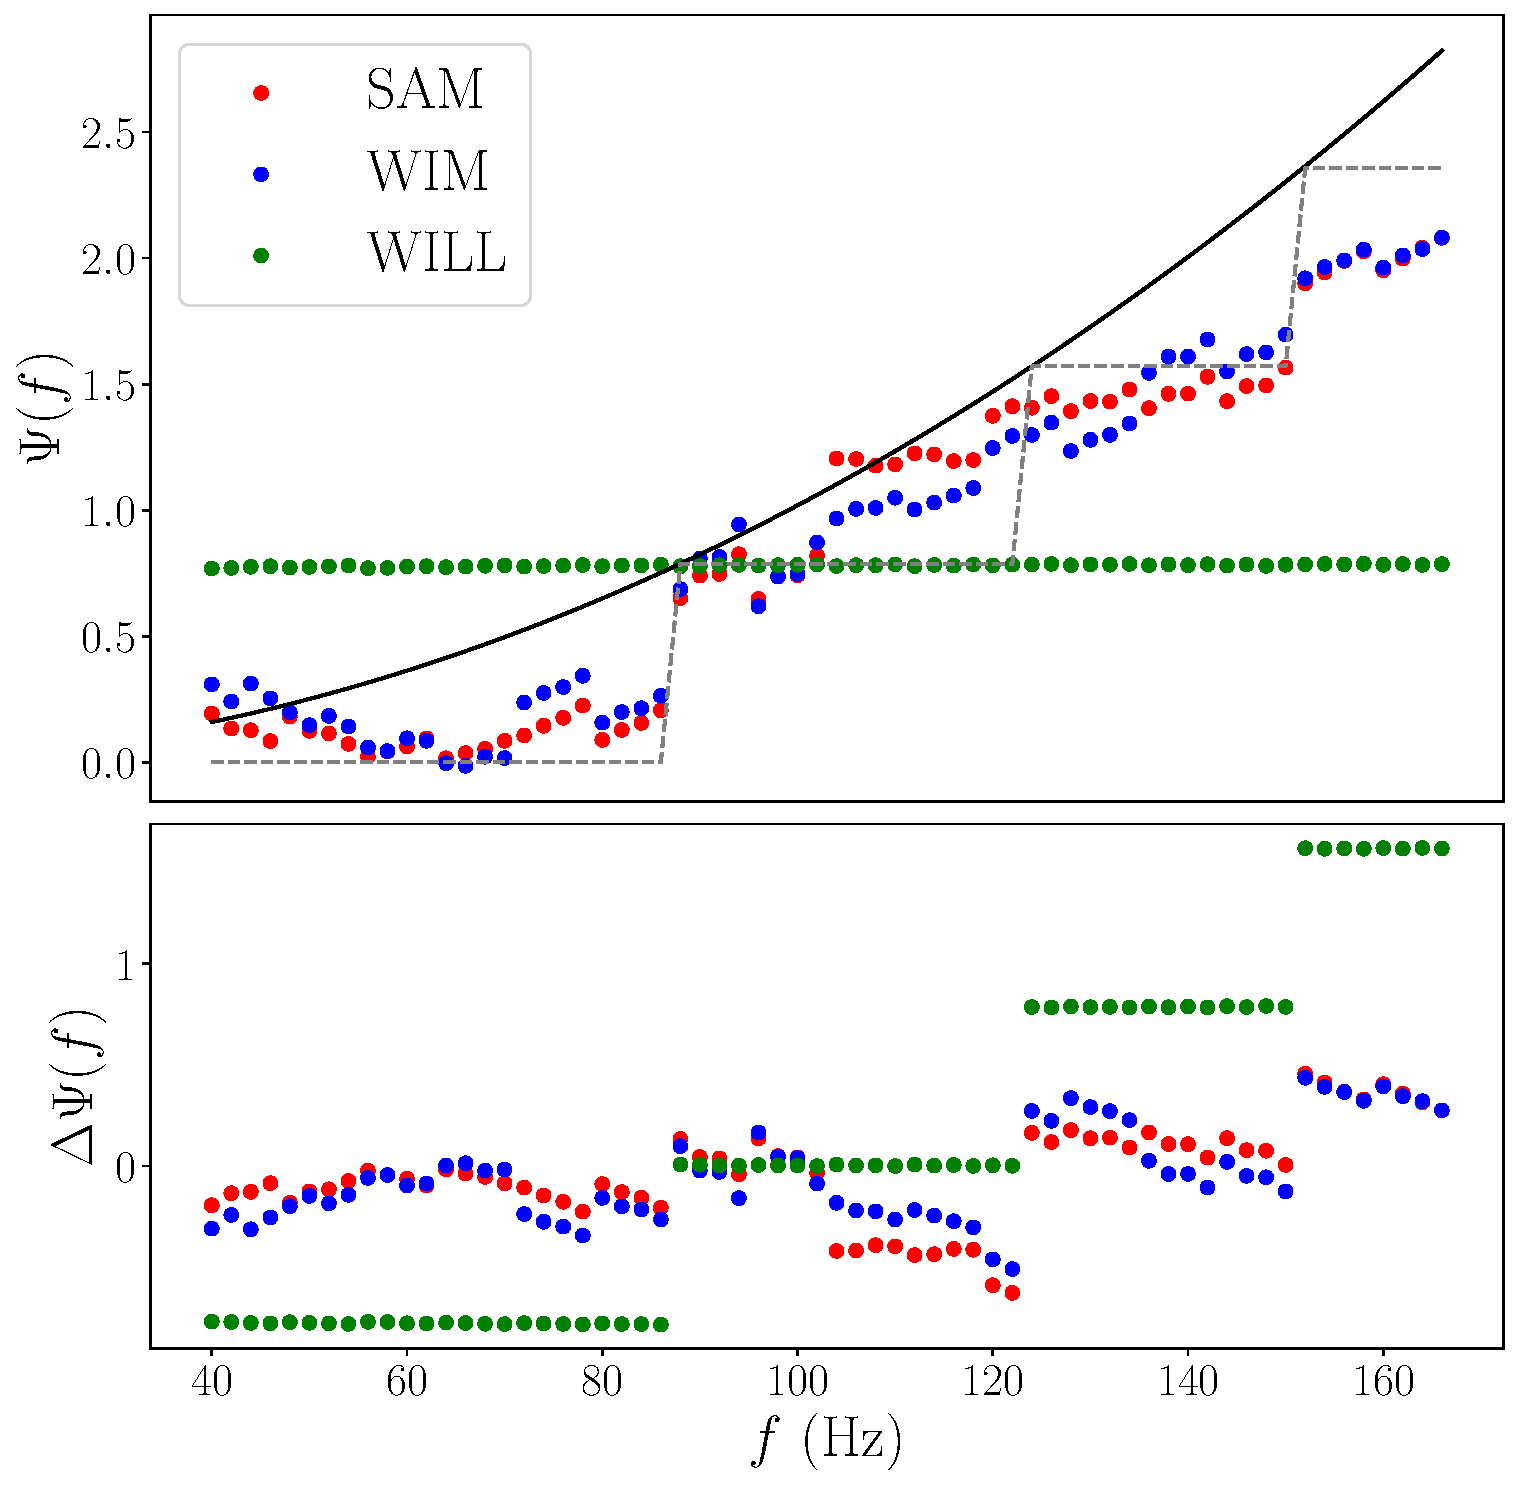
\includegraphics[width=\textwidth]{im/SAM_WIM_WILL_F2_new}
\caption{Comparing extracted phase functions for $\Psi(f) \sim f^2$ ($L=6$, $m=3$, 600 epochs)}
\end{figure}
\end{column}
\end{columns}
\end{frame}

\begin{frame}
\frametitle{Comparing SAM, WIM, and WILL}
\begin{columns}
\begin{column}{0.5\textwidth}
\begin{table}
\begin{tabular}{c || c| c| c }
& SAM & WIM & WILL \\ \hline \hline 
$\mu$ &  \textbf{6.8e-2} & 8.4e-2 & 7.6e-2 \\
$\sigma$ &  1.8e-1 & \textbf{1.2e-1} & 2.6e-1 \\
$\epsilon$  &  4.5e-2 & 1.8e-1 & \textbf{7.3e-3 } \\
$\chi$ &  7.4e-2 & 1.0e-1 & \textbf{6.2e-2} \\ \hline 
$\Omega$ &  \textbf{2.75} & 2.07 & 2.48
\end{tabular}
\caption{Comparing loss function metrics for $\Psi_\text{H23}$ ($L=6$, $m=3$, 600 epochs)}
\end{table}
\end{column}
\begin{column}{0.5\textwidth}
\begin{figure}
\centering 
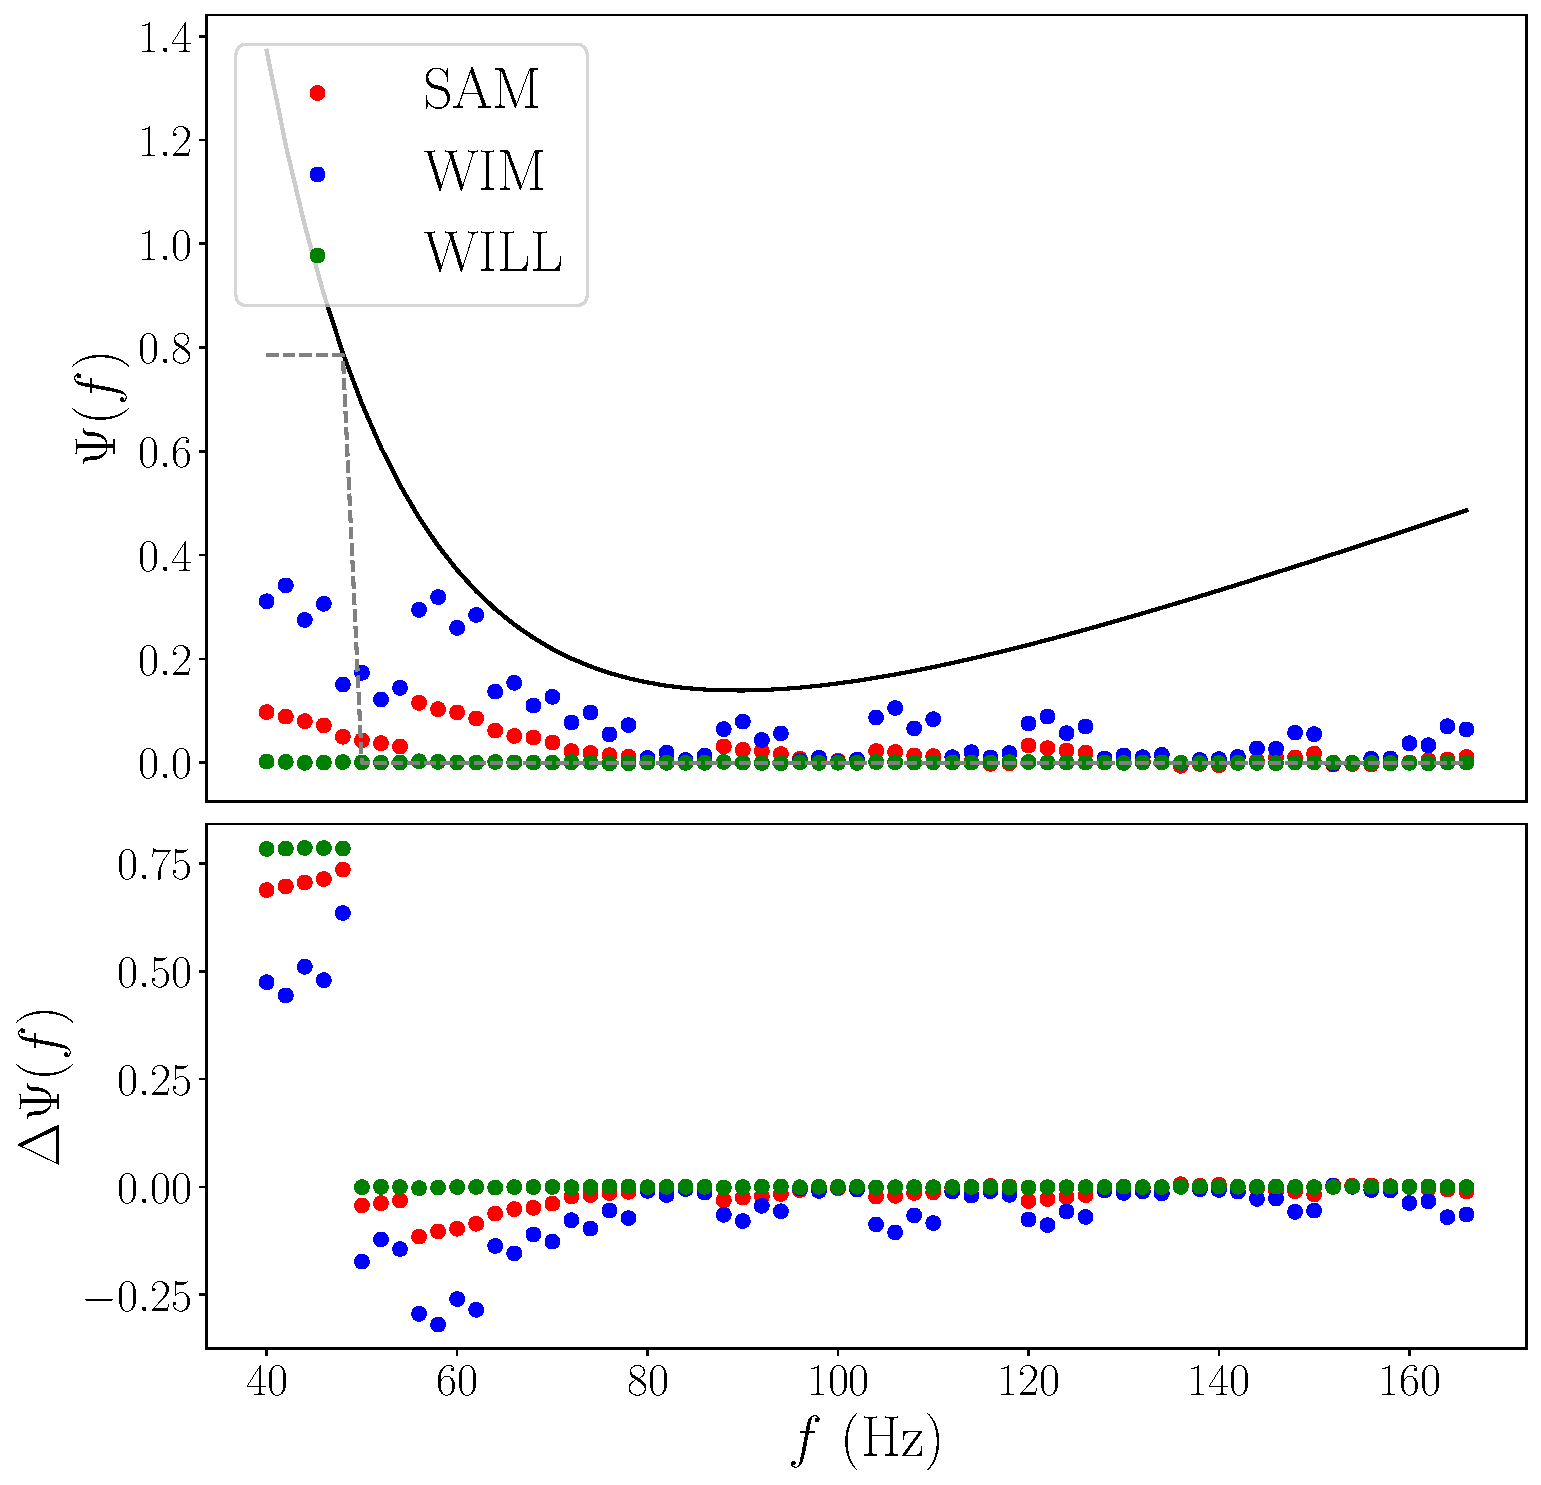
\includegraphics[width=\textwidth]{im/SAM_WIM_WILL_H_new}
\caption{Comparing extracted phase functions for $\Psi_\text{H23}$ ($L=6$, $m=3$, 600 epochs)}
\end{figure}
\end{column}
\end{columns}
\end{frame}

\begin{frame}
\frametitle{Other Approaches}
\begin{itemize}
\item Attempts to define a loss function based directly on $\hat{Q}^\dagger \hat{R} \hat{Q}$, e.g. minimising $\chi$, were \alert{unsuccessful} 
\item This is due to the \emph{qiskit machine learning} environment being build around \alert{sampler primitives} which return quasi-probabilities instead of probability amplitudes 
\item Thus, phases cannot be directly taken into account for gradient calculation 
\item A possible work-around could be to switch to a QCNN based on an \alert{estimator primitive}, which calculates the expectation value of an observable w.r.t to the state prepared by the network 
\item This would require the construction of an \alert{appropriate operator} (note: qiskit supports non-Hermitian observables) 
\end{itemize}
\end{frame}

\begin{frame}
\frametitle{An Estimator-based PQC}
\begin{itemize}
\item Let $\ket{\tilde{\phi}}$ be the $n$-qubit state produced by the PQC:
\begin{equation}
\ket{\tilde{\phi}}= \sum_k \tilde{A}(k) e^{i \tilde{\Psi}(k)} \ket{k}
\end{equation}
\item The desired output state is 
\begin{equation}
\ket{\phi}= \sum_k A(k) e^{i \Psi(k)} \ket{k}
\end{equation}
\item An estimator-based optimiser calculates the loss and gradients for each epoch based on the expectation value 
\begin{equation} \mathbb{E}(\tilde{\phi}) \equiv \braket{\tilde{\phi}| \hat{O}| \tilde{\phi}} = \sum_{k, k'} \tilde{A}(k')\tilde{A}(k) \exp \left(i \left[ \tilde{\Psi}(k) - \tilde{\Psi}(k') \right] \right) \braket{k' | \hat{O}| k}, 
\end{equation}
for some operator $\hat{O}$
\end{itemize}
\end{frame}

\begin{frame}
\frametitle{An Estimator-based PQC}
\begin{itemize}
\item Now construct $\hat{O}$ such that 
\begin{equation}
\braket{k' | \hat{O} | k} \equiv \frac{1}{A(k')A(k)}  \exp \left( - i \left[ \Psi(k) - \Psi(k') \right] \right)
\end{equation}
for $A(k), A(k') \neq 0$
\item Then 
\begin{equation}
\mathbb{E}(\phi)= \sum_{k,k'} 1 =2^{2n}
\end{equation}
so that we can train the network to generate $\ket{\phi}$ by minimising $|1-\mathbb{E}(\tilde{\phi}) / 2^{2n}|$
\item \alert{This is highly speculative} and computationally very expensive even for simple PQCs due to the way custom operators are handed in qiskit
\item Thus, \alert{estimator-based PQCs cannot feasibly replace the sampler-based QCNN}
\end{itemize}
\end{frame}

\begin{frame}
\frametitle{Loss Function: Conclusion}
\begin{itemize}
\item The design of the \emph{qiskit machine learning} library \alert{constrains the customisability} of loss functions, in particular relating to phases 
\item Thus, \alert{loss functions based directly on the extracted phase} factors are (apparently) \alert{impossible} 
\item Within the limits of these constraints the \alert{best} possible loss function seems to be \alert{SAM} 
\item Beyond the unsuccessful attempts of WIM and WILL no further  \emph{ans\"atze} for loss functions come to mind 
\item For the time being, the search for an improved loss function will be \alert{put on hold}
\end{itemize}
\end{frame}

\section{Investigating Phase Extraction}

\begin{frame}
\frametitle{Investigating Phase Extraction}
\begin{itemize}
\item The operator $\hat{Q}$ is defined via 
\begin{equation}
\hat{Q} \ket{j} \ket{0} = \ket{j} \ket{\Psi(j)}
\end{equation}
\item This leaves its action on more general input states $\ket{j}\ket{k}$ (with $\ket{k} \neq \ket{0}$) \alert{undetermined} 
\item Thus, there is a \alert{family} $\mathcal{Q}$ of valid implementations of $\hat{Q}$ with $|\mathcal{Q}|=(n+m)^2 -n$ 
\item We can represent a flawed implementation, $\tilde{Q}$, of $\hat{Q}$ via $\tilde{Q} = \hat{Q} + \lambda \hat{P}$ so that 
\begin{equation}
\tilde{Q}\hat{R} \tilde{Q} = \hat{Q}^\dagger \hat{R} \hat{Q} + \lambda \left[ \hat{Q}^\dagger  \hat{R} \hat{P} + \hat{P}^\dagger \hat{R} \hat{Q}\right] + \lambda^2 \left[ \hat{P}^\dagger \hat{R} \hat{P} \right]
\end{equation}
\item Beyond these very general observations \alert{no analytical insight into the problem was gained}
\end{itemize}
\end{frame}

\section{Mitigating Barren Plateaus}

\begin{frame}
\frametitle{Mitigating Barren Plateaus}
\begin{itemize}
\item The most important strategy to mitigate barren plateaus seems to be a so-called \alert{warm start}, also known as \alert{smart initialisation}
\item 
\end{itemize}

GENERATE A FEW PLOTS FOR GRAD AND VAR GRAD FOR DIFFERENT n and m...: diagonose problem: plot var(grad) and |grad| as function of epoch for different n+m (maybe go down with n  as well)...



most important seems to be `smart initialisation' or `warm-start'

\end{frame}



\section{Next Steps}

\begin{frame}
\frametitle{Next Steps}
\begin{itemize}
\item Keep re-writing code for easier implementation of barren plateau mitigation techniques
\item ...
\end{itemize}
\end{frame}



\end{document}